\section{Map\-Object Class Reference}
\label{classMapObject}\index{MapObject@{MapObject}}
{\tt \#include $<$mapobject.hpp$>$}

Inheritance diagram for Map\-Object::\begin{figure}[H]
\begin{center}
\leavevmode
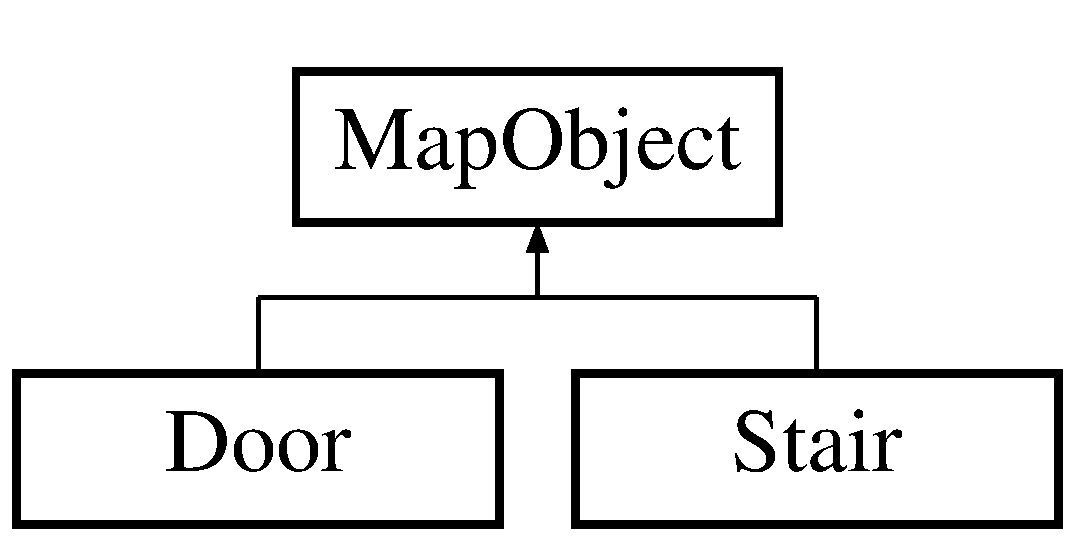
\includegraphics[height=2cm]{classMapObject}
\end{center}
\end{figure}
\subsection*{Public Member Functions}
\begin{CompactItemize}
\item 
virtual QString {\bf get\-Class\-Name} () const =0
\item 
int {\bf get\-Tile} () const 
\item 
virtual bool {\bf is\-Obstacle} () const 
\item 
virtual bool {\bf is\-Bulletproof} () const 
\item 
virtual bool {\bf is\-Visionproof} () const 
\end{CompactItemize}
\subsection*{Protected Attributes}
\begin{CompactItemize}
\item 
int {\bf tile}
\end{CompactItemize}


\subsection{Member Function Documentation}
\index{MapObject@{Map\-Object}!getClassName@{getClassName}}
\index{getClassName@{getClassName}!MapObject@{Map\-Object}}
\subsubsection{\setlength{\rightskip}{0pt plus 5cm}virtual QString get\-Class\-Name () const\hspace{0.3cm}{\tt  [pure virtual]}}\label{classMapObject_a0}




Implemented in {\bf Door} {\rm (p.\,\pageref{classDoor_a2})}, and {\bf Stair} {\rm (p.\,\pageref{classStair_a2})}.\index{MapObject@{Map\-Object}!getTile@{getTile}}
\index{getTile@{getTile}!MapObject@{Map\-Object}}
\subsubsection{\setlength{\rightskip}{0pt plus 5cm}int get\-Tile () const}\label{classMapObject_a1}


\index{MapObject@{Map\-Object}!isBulletproof@{isBulletproof}}
\index{isBulletproof@{isBulletproof}!MapObject@{Map\-Object}}
\subsubsection{\setlength{\rightskip}{0pt plus 5cm}bool is\-Bulletproof () const\hspace{0.3cm}{\tt  [virtual]}}\label{classMapObject_a3}




Reimplemented in {\bf Door} {\rm (p.\,\pageref{classDoor_a4})}.\index{MapObject@{Map\-Object}!isObstacle@{isObstacle}}
\index{isObstacle@{isObstacle}!MapObject@{Map\-Object}}
\subsubsection{\setlength{\rightskip}{0pt plus 5cm}bool is\-Obstacle () const\hspace{0.3cm}{\tt  [virtual]}}\label{classMapObject_a2}




Reimplemented in {\bf Door} {\rm (p.\,\pageref{classDoor_a3})}.\index{MapObject@{Map\-Object}!isVisionproof@{isVisionproof}}
\index{isVisionproof@{isVisionproof}!MapObject@{Map\-Object}}
\subsubsection{\setlength{\rightskip}{0pt plus 5cm}bool is\-Visionproof () const\hspace{0.3cm}{\tt  [virtual]}}\label{classMapObject_a4}




Reimplemented in {\bf Door} {\rm (p.\,\pageref{classDoor_a5})}.

\subsection{Member Data Documentation}
\index{MapObject@{Map\-Object}!tile@{tile}}
\index{tile@{tile}!MapObject@{Map\-Object}}
\subsubsection{\setlength{\rightskip}{0pt plus 5cm}int {\bf tile}\hspace{0.3cm}{\tt  [protected]}}\label{classMapObject_p0}




The documentation for this class was generated from the following files:\begin{CompactItemize}
\item 
{\bf mapobject.hpp}\item 
{\bf mapobject.cpp}\end{CompactItemize}
